\section{Gaia-X}
\label{sec:grundlagen:gaia-x}
Europas Plan für digitale Souveränität besteht aus der Cloud- sowie Datenselbstbestimmung.
Cloudsouveränität ist wichtig, um Services zu nutzen, die europäischen Regulierungen entsprechen \cite{Braud2021}.
Gaia-X ist hierfür die Initiative, einen freien Software Stack für Kontrolle, Governance und Erstellung gemeinsamer
Regeln und Richtlinien zu entwickeln \cite{Bonfiglio2021}. 
Dieser Stack soll auf allen bestehenden Cloudtechnologien anwendbar sein, um Transparenz, Souveränität und 
Interoperabilität bei Datenübermittlung und Dienstleistungen zu erreichen \cite{Bonfiglio2021}.

\subsection{Architektur}
\label{subsec:gaia-x:architektur}
\paragraph{Design Prinzipien}
Die Gaia-X Architektur beruht auf den folgenden Design Prinzipien:

\subparagraph{Föderationen}
Föderalisierte Systeme beschreiben autonome Einheiten, die durch eine spezifizierte Reihe von Normen,
Frameworks und Regeln verbunden sind.
Das Prinzip soll mit einer minimalen Anzahl an Vorgaben die Interoperabilität und den Informationsaustausch
zwischen den einzelnen Einheiten der Föderation ermöglichen. 
Dabei soll gleichzeitig das Höchstmaß an Autonomie gewährleistet werden \cite{GaiaXArchitecture2021}.
Durch Föderationen können Serviceanbieter ihre Infrastruktur auf vertrauenswürde Weise miteinander verbinden,
um ein verteiltes Cloud-Modell anzubieten \cite{Bonfiglio2021}.

\subparagraph{Dezentralisierung}
Mitglieder einer Föderation sollen selbstorganisiert, ohne zentrale Kontrolle, operieren.
Das Föderationsprinzip ermöglicht diese Selbstorganisation durch die Bereitstellung eines Netzworks
zur Interaktion mit anderen Gaia-X Teilnehmern \cite{GaiaXArchitecture2021}.

\subparagraph{Offenheit}
Eine offene Architektur ermöglicht das einfache Hinzufügen, Aktualisieren und Änderung von Komponenten, sowie
Einblicke in alle Teile der Architektur und proprietäre Nutzung von Software.
Dadurch ist Gaia-X offen für zukünftige Innovationen und Standards und fortschreitende Technologie \cite{GaiaXArchitecture2021}.

\begin{figure}[h]
  \centering
  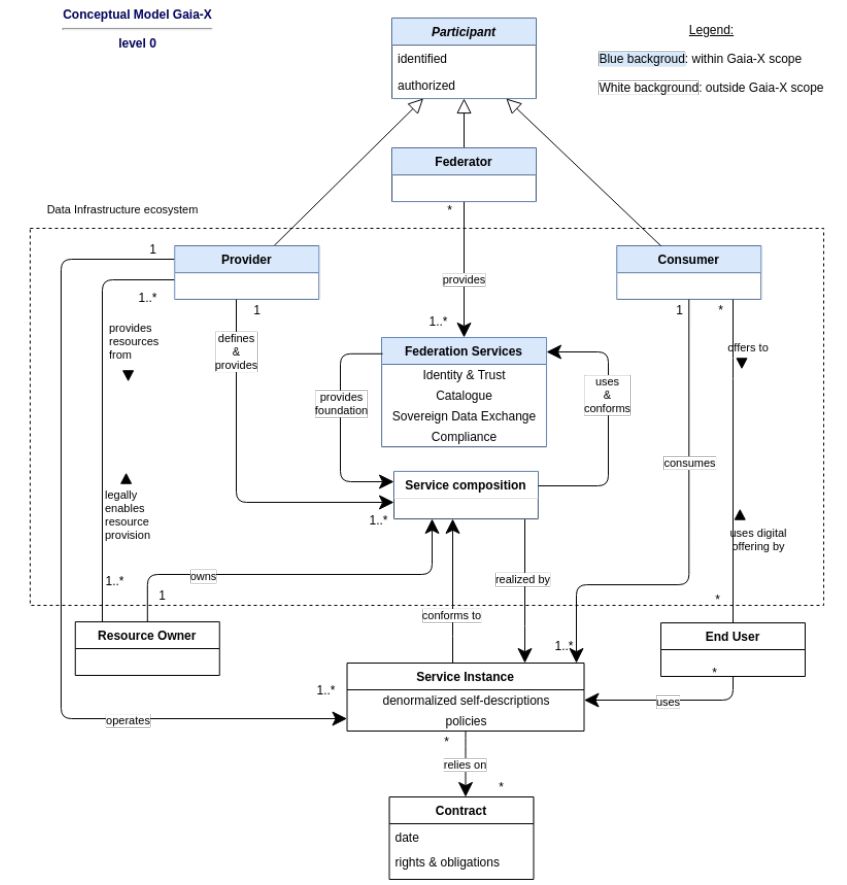
\includegraphics[width=\textwidth]{gfx/chapters/2_grundlagen/gaia-x-architecture.png}
  \caption{Konzeptuelles Modell der Gaia-X Architektur}
  \source{\cite{GaiaXArchitecture2021}}
  \label{fig:gaia-x-concept-architecture}
\end{figure}

\paragraph{Architekturkonzept}
In \ref{fig:gaia-x-concept-architecture} wird das Architekturkonzept, sowie den Umfang von Gaia-X verdeutlich.
Der obere Teil des Modells zeigt die verschiedenen Akteure innerhalb von Gaia-X, während der
untere Teil den Umfang und die Beziehung der Akteuere außerhalb von Gaia-X darstellt.

\subparagraph{Participants}
Participants sind Teilnehmer innerhalb von Gaia-X. 
Dabei können sie eine oder mehrere Rollen einehmen: Föderalist, Anbieter oder Konsument \cite{GaiaXArchitecture2021}.

\subparagraph{Anbieter}
Anbieter sind Teilnehmer, die Ressourcen im Gaia-X Ecosystem bereitstellen. Zudem stellt
ein Anbieter Services mit deren allgemeinen Geschäftsbedingungen und technische Richtlinien bereit \cite{GaiaXArchitecture2021}.

\subparagraph{Föderalist}
Ein Föderalist ist für die Implementierung der Föderationsservices (\ref{subsec:gaia-x:federationservices}) 
sowie für die Koordination der Teilnehmer zuständig \cite{GXFS2021}.

\subparagraph{Konsument}
Konsumenten nutzen Services im Gaia-X Ecosystem um digitale Angebote für Kunden zu ermöglichen \cite{GaiaXArchitecture2021}.

\subsection{Föderationsservices}
\label{subsec:gaia-x:federationservices}
Föderationsservices können als minimale technische Anforderungen zur Operativität der Föderation angesehen werden \cite{GXFS2021}.
Dabei werden Services definiert, welche zur Erfüllung der Ziele von Gaia-X, Vertrauen und Interoperabilität
aufzubauen, sowie die Sicherstellung von Datensouveränität für Teilnehmer zu gewährleisten, beitragen \cite{GXFS2021}.
Zum Start des Gaia-X Projekts werden die folgenden vier Services definiert:

\paragraph{Identität und Vertrauen}
Teilnehmer einer Föderation nutzen diesen Service, um Authentifizierung und Authorisierung innerhalb der Föderation zu nutzen \cite{GXFS2021}.

\paragraph{Föderalisierter Katalog}
Der Katalog dient als zentrales Repository einer Föderation.
Er ermöglicht Teilnehmern das Finden von Informationen und Dienste anderer Föderationsteilnehmer durch Nutzung von
\emph{Self-Descriptions} (\ref{sec:gaia-x-einbettung:gaia-x-katalog}) \cite{GXFS2021}.

\paragraph{Datensouveränität}
Dieser Service hilft Teilnehmer der Föderation Kontrolle und einen Überblick über ihre Daten zu behalten.
Dabei werden Verfahren implementiert, um Transparenz und Kontrolle über Datennutzung zu definieren \cite{GXFS2021}.

\paragraph{Konformität}
Konformitätsservices ermöglichen die Überprüfung der gemeinsamen Services in einer Föderation auf Einhaltung
von Gaia-X Prinzipien wie Datensicherheit \cite{GXFS2021}.
